% 第 19 题抛物线图：按固定源 PDF 矢量路径换算（1 pt → 0.03515 cm）。
% 原点取 O（抛物线顶点，源页 (670.24, 226.48) pt），y 向上。
% 抛物线线宽 0.8pt（其余图元 2 倍），按源三采样点拟合式 y² = 28.35 x′ 绘制（绘制比例下 p/2 ≈ 7.09 pt）；
% 源为示意画法（F 距原点 22.67 pt ≈ 3.2 倍半焦距、FN 与 AB 实测 87.2°），照源复刻不校正。
% 直线 4 条：A–B（焦点弦所在直线，仅连两点）、B–N（水平）、A–N、F–N；
% x 轴左 28.33 右至箭头尖点 99.18；y 轴下 56.67 上至箭头尖点 56.68。
% 各点旁标注（照源字形框中心）；M 处无独立标记（为 A–N 与 x 轴交点，源仅标字母）。
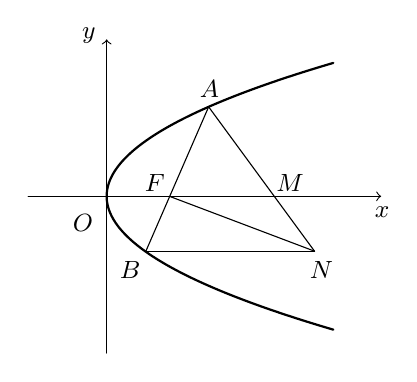
\begin{tikzpicture}[line cap=round,line join=round,font=\small,x=0.03515cm,y=0.03515cm]
% 坐标轴
\draw[->] (-28.33,0)--(99.18,0);
\draw[->] (0,-56.67)--(0,56.68);
% 抛物线（线宽 0.8，与源一致）
\draw[line width=0.8pt] plot[domain=-48.18:48.18,samples=121] ({\x*\x/28.35},{\x});
% ===== 直线段 =====
\draw (14.17,-19.83)--(36.84,32.31);   % A–B
\draw (14.17,-19.83)--(75.09,-19.83);  % B–N（水平）
\draw (36.84,32.31)--(75.09,-19.83);   % A–N
\draw (22.67,0)--(75.09,-19.83);       % F–N
% ===== 标注（照源字形框中心，显式坐标）=====
\node[anchor=center,inner sep=0] at (-6.39,58.10) {\(y\)};
\node[anchor=center,inner sep=0] at (37.11,38.74) {\(A\)};
\node[anchor=center,inner sep=0] at (17.39,4.73) {\(F\)};
\node[anchor=center,inner sep=0] at (66.30,4.73) {\(M\)};
\node[anchor=center,inner sep=0] at (99.47,-5.58) {\(x\)};
\node[anchor=center,inner sep=0] at (-8.58,-9.66) {\(O\)};
\node[anchor=center,inner sep=0] at (8.50,-26.45) {\(B\)};
\node[anchor=center,inner sep=0] at (77.64,-26.45) {\(N\)};
\end{tikzpicture}
